\documentclass[12pt,a4paper,oneside,draft]{book}
\usepackage{hyperref}
\usepackage{graphicx}

\begin{document}

\title{Infotv-dev}
\author{Aleksi Salmela}
\date{\today}
\maketitle

\tableofcontents

\chapter{Introduction}
The projects goal is to show current news for the visitors. The project consists of main page and admin panel. The main page only shows the current news and the admin panel allows contributors to write new news pages to the main page.

The project allows organization to show relevant news about their current projects to the their employees. The admin panel must allow adding, listing and removing of the fonts, themes and pages.

Most of the development will happen on my local computer, but I will update the progress to the users-server before weeks deadline. I will implement the project in php and the project most likely will integrate the tinymce text editor into the admin panel.

The project won't require javascript and I will try to fallback to simple html forms if the javascript is not present. The web pages will require obviously css and html support from the browser and I try to write the code so that it will at least somehow work in older browsers, but it may not look as pretty.

I will propably first use Mysql database for the project, but I may migrate to the Postgres if there is problems with Mysql. To allow better portability I won't use sql procedures nor some other exotic features.

\url{http://www.tinymce.com/}

\chapter{Overview}
\section{Users}
\begin{description}
  \item[Anyone]      Anyone who knows the address of the web page.
  \item[Contributor] User who has permission to write new pages to the system.
  \item[Admin]       User who has right to everything in the system.
\end{description}

\section{Use cases}
\begin{figure}
\centering
%%\input{use_cases.tex}
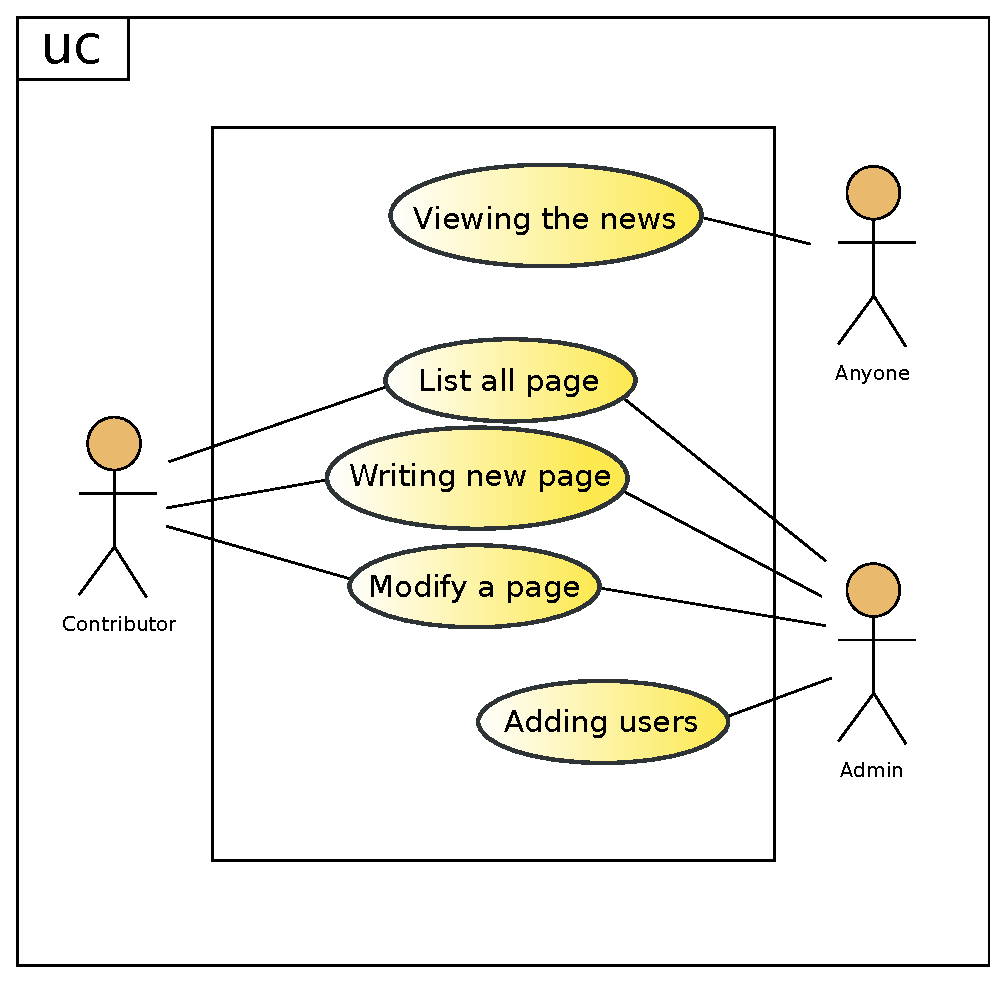
\includegraphics[width=\textwidth]{use_cases.eps}
\caption{Use case}
\end{figure}

\subsection{Anyone}
\begin{description}
  \item[Viewing the news] \hfill \\
	Anyone can view the pages written to the system \hfill \\
	Example: If employee wants to know if there has been new breakthroughs in some project he can go to the website and see the todays news.
\end{description}

\subsection{Contributor}
\begin{description}
  \item[Writing new page] \hfill \\
	Contributor can login to the system and click a button to create new page. The admin panel then shows a input box for the title of the news and a text box for writing the content of the news. The contributor has to choose a theme/category for the news or leave it to the default. \hfill \\
	Example: The contributor can write a piece of news about the project xyz.
  \item[Modify a page] \hfill \\
	 The contributor must be able to modify the pages that they have written. \hfill \\
	Example: The contributor can fix a typo in the existing piece of news.
  \item[List all pages] \hfill \\
	 The contributor must be able to see list of all the pages and sort the my category, author, date or name. \hfill \\
	Example: The contributor can find out if somebody else has already written about a event.
\end{description}

\subsection{Admin}
\begin{description}
  \item[Editing page] \hfill \\
	The admin can modify any page in the system \hfill \\
	Example: If the admin notices performance problems in some news page, then admin can modify the page so that it will load faster.
  \item[Adding users] \hfill \\
	The admin can add new users to the system \hfill \\
	Example: If there is new contributor the admin can give him a new account.
\end{description}

\end{document}
